\documentclass[lettersize,journal]{IEEEtran}
\usepackage{amsmath,amsfonts}
\usepackage{algorithmic}
\usepackage{array}
\usepackage[caption=false,font=normalsize,labelfont=sf,textfont=sf]{subfig}
\usepackage{textcomp}
\usepackage{stfloats}
\usepackage[ngerman]{babel}
\addto\captionsngerman{\renewcommand{\figurename}{Abb.}}
\addto\extrasngerman{\def\figureautorefname{Abb.}}
\usepackage{float}
\usepackage{url}
\usepackage{verbatim}
\usepackage{placeins}
\usepackage{graphicx}
\usepackage{caption} % In Präambel
\usepackage{cuted}
\usepackage{package}
\hyphenation{op-tical net-works semi-conduc-tor IEEE-Xplore}
\def\BibTeX{{\rm B\kern-.05em{\sc i\kern-.025em b}\kern-.08em
		T\kern-.1667em\lower.7ex\hbox{E}\kern-.125emX}}
\usepackage{balance}


\begin{document}
\title{Implementierung eines Zero Trust Network}
\author{
	Marc Reuschenberg, Jürgen Güsting, Prof. Dr. rer. nat. Marko Schuba\\
	EXPLETO GmbH, Zieglersteg 7, Aachen \\
	FH Aachen, University of Applied Sciences, Eupenerstr. 70, Aachen\\
	marc.reuschenberg@alumni.fh-aachen.de
}
\markboth{PRAXISPROJEKTBERICHT: Implementierung eines Zero Trust Network, Juni 2025}
{}
\IEEEaftertitletext{%
	\vspace{-2em}
	\begin{center}
		\begin{minipage}[c]{0.3\textwidth}
			\centering
			
\includegraphics[width=\linewidth]{expleto-logo-primary.png}
		\end{minipage}
		\hspace{1em}
		\begin{minipage}[c]{0.3\textwidth}
			\centering
			
\includegraphics[width=\linewidth]{FHAachen-logo2010.png}
		\end{minipage}
	\end{center}
	\vspace{1cm}
}

\maketitle

\begin{abstract}
In Zeiten von Cloud-Diensten, mobilen Arbeitsplätzen und hybriden IT-Infrastrukturen stößt das perimeterbasierte Sicherheitskonzept immer mehr an seine Grenzen. Das Zero Trust Modell bietet einen  Sicherheitsansatz, bei dem grundsätzlich kein Zugriff als vertrauenswürdig gilt. Jeder Zugriff muss somit geprüft werden, ganz egal, ob dieser innerhalb oder außerhalb des internen Firmennetzwerkes geschieht. Ziel dieser Arbeit ist es, die Zero Trust Prinzipien zu verstehen und technische Maßnahmen zu finden, damit ein Netzwerk nach Zero Trust konstruiert werden kann. Das Ergebnis ist ein Netzwerk, welches auf den Konzepten Identitäts- und Zugriffsmanagement, Netzwerksegmentierung, Gerätesicherheit, Netzwerkzugriffskontrolle, Überwachung und Monitoring beruht.
\end{abstract}
\begin{IEEEkeywords}
	IT-Sicherheit, ZTN, Implementierung, Identitäts- und Zugriffsmanagement, Netzwerksegmentierung, Gerätesicherheit, Netzwerkzugriffskontrolle, Überwachung und Monitoring.
\end{IEEEkeywords}
\section{Einleitung}
Netzwerke bilden heute die Basis für moderne IT-Infrastrukturen und sind aus Sicht der Unternehmen nicht mehr wegzudenken \cite{Afolalu.2025}. Sie ermöglichen den gemeinsamen Zugriff auf Ressourcen und bieten Kommunikationsmöglichkeiten zwischen Mitarbeitern, Abteilungen und verschiedenen Standorten \Cites[3]{Schreiner.2023}. Ein leistungsfähiges und sicheres Netzwerk ist daher essenziell für den geschützten und stabilen Betrieb unternehmerischer Prozesse. 
Netzwerke werden auf Grundlage von Sicherheitsmodellen konzipiert. Ein traditionelles Sicherheitsmodell basiert dabei auf dem sogenannten Perimeter-Schutz. Dabei wird davon ausgegangen, dass das interne Netzwerk vertrauenswürdig ist und nur externe Zugriffe besonders abgesichert werden müssen. Der Schutz konzentriert sich daher hauptsächlich auf die externen Grenzen des Netzwerkes, während dem internen Netzwerk ein gewisses Maß an Vertrauen entgegengebracht wird \cite{cloudflare.com.2025}.
Dieses Modell stößt jedoch in Zeiten der wachsenden Bedeutung von Cloud-Diensten, mobilen Arbeitsplätzen und hybriden IT-Infrastrukturen immer mehr an seine Grenzen \cite[29]{Riepen.2022131}. Klare Trennungen zwischen internen und externen Netzwerken sind in modernen Unternehmen oftmals schwer zu erkennen. Angriffe erfolgen nicht nur noch von außen, sondern auch durch kompromittierte Geräte im internen Unternehmensnetzwerk \cite{Horne.2021}. Vor diesem Hintergrund gewinnt das Zero Trust Modell immer mehr an Bedeutung.\\
Ziel dieser Arbeit ist es, den aktuellen Stand des Zero Trust Konzepts zu analysieren und auf dieser Grundlage ein eigenes Zero Trust Network zu entwerfen und praktisch zu implementieren. Die Umsetzung erfolgt in einer Testumgebung und orientiert sich dabei an den Kernprinzipien von Zero Trust.

\section{Entwicklung des Sicherheitsmodells Zero Trust}
Zero Trust ist kein neu erfundenes Schlagwort. Vielmehr ist die erstmalige Verwendung dieses Begriffes zurückzuführen bis ins Jahr 1994 \cite[8]{BundesamtfurSicherheitinderInformationstechnik.2023}. Genannt von Stephen Paul Marsh, fand sich der Begriff in seiner Doktorarbeit zur Computersicherheit an der Universität Stirling wieder \cite[8]{BundesamtfurSicherheitinderInformationstechnik.2023}. Verstärkt betrachtet wurde der Begriff und sein Konzept dann aber erst in den 2000er Jahren. Zunächst fand sich das Konzept hinter Zero Trust in einer Diskussion vom Jericho Forum wieder. Ausgangslage war das Erschaffen eines neuen Sicherheitsverständnisses hin zu einer De-Perimeteraisation \cite{Fox.2022}. Im Jahr 2010 veröffentlichte ein Forrester-Analyst namens John Kindervag ein Whitepaper, in dem er den Begriff Zero Trust mit den neu entworfenen Sicherheitsmodellen des Jericho Forums in Verbindung brachte. Dieses Whitepaper ist heute bekannt unter dem Namen No More Chwey Centers. Über die Jahre wurde das Konzept immer weiterentwickelt, bis Google 2010 mit dem Entwurf einer Zero Trust Architektur für seine Infrastruktur begann. Dieser Schritt war auf die erfolgreiche Operation Aurora zurückzuführen, die ein spezialisierter und gezielter Angriff auf Google und seine Infrastruktur war. Das Projekt wurde unter dem Namen BeyonCorp bekannt und brachte die gewonnenen Erkenntnisse 2014 in einem Forschungsbericht zum Vorschein. 2019 festigte das US National Institute of Standards and Technology (NIST) die Wichtigkeit von Zero Trust, indem es eine Anleitung für Zero Trust publizierte. In dieser Ausarbeitung wurden drei Kerprinzipien von Zero Trust genannt:
\begin{itemize}
	\item Kein implizites Vertrauen
	\item Minimale Rechtevergabe
	\item Dynamische Zugriffsentscheidung
\end{itemize}
Diese Prinzipien gelten seither und werden je nach Literatur um einige weitere Prinzipien ergänzt  \cite{BundesamtfurSicherheitinderInformationstechnik.2023}.
Bei Zero Trust handelt es sich heute um keine einzelne Lösung, die es zu kaufen oder zu implementieren gibt. Vielmehr ist Zero Trust eine Philosophie, die es mit der Technik zu vereinen gilt. Auch wenn Zero Trust eine mögliche Ausrichtung des Unternehmens für mehr Sicherheit ist, müssen trotzdem hinsichtlich des Aufwandes, der Pflege, Wartung und Risiken in Form von Single Point of Failure und Persönlichkeitsrechte abgewogen werden \cite{Fox.2022}.
Zero Trust wird ständig verfeinert und überprüft. Es findet einen immer höheren Stellenwert in der Informationssicherheit. 

\section{Eigener Ansatz}
Unter Betrachtung der zuvor genannten Prinzipien von Zero Trust ergeben sich Anforderungen an ein zu implementierendes Zero Trust Network. Daher fokussiert sich die Arbeit insbesondere auf die Umsetzung folgender technischer Maßnahmen:

\begin{itemize}
	\item Identitäts- und Zugriffsmanagement
	\item Netzwerksegmentierung
	\item Gerätesicherheit
	\item Netzwerkzugriffskontrolle
	\item Überwachung und Monitoring
\end{itemize}
Durch die Umsetzung dieser Maßnahmen sollen die Prinzipien von Zero Trust im zu konzipierenden Netzwerk wiederzufinden sein. Die einzelnen Schlüsselkonzepte erfüllen zum Teil mehrere Prinzipien von Zero Trust.

\subsection{Identitäts- und Zugriffsmanagement}
Das Identitäts- und Zugriffsmanagement (IAM) sorgt dafür, dass Zugriffe auf bestimmte Ressourcen nur von bestimmten Identitäten durchgeführt werden dürfen. Einzeln betrachtet sorgt das Identitätsmanagement dafür, dass Identitäten bekannt und gepflegt sind. Mittels dieser Identitäten kann das Zugriffsmanagement unter Prüfung von vorher definierten Voraussetzungen den Zugang zu Ressourcen gewähren \cite{Faber.2021}. Auf Grundlage dieser Betrachtung können den Nutzern des Netzwerkes verschiedene Merkmale mitgegeben werden. Diese Merkmale beziehen sich auf Eigenschaften des Nutzers oder seines Endgeräts. Beispiele dafür können das aktuelle Betriebssystem sein, die Zugehörigkeit zu einer Domäne und in welcher Gruppe sich der Nutzer befindet. Anhand dieser Eigenschaften kann das Zugriffsmanagement die Zugriffe feiner steuern. Die Entscheidung, ob ein Nutzer auf eine bestimmte Ressource zugreifen darf, wird so nicht nur noch anhand von Quell-/Ziel-IP-Adresse und Quell-/Zielport gesteuert. Das Konzept hinter dem Identitäts- und Zugriffsmanagement verfolgt zum großen Teil die Umsetzung des 'Kein implizites Vertrauen' -Prinzips.

\subsection{Netzwerksegmentierung}
Bei der Netzwerksegmentierung wird ein Netzwerk in mehrere kleinere logische Einheiten aufgeteilt. Eine Segmentierung des Netzwerkes ist auf physischer und virtueller Schicht möglich. Auf physischer Ebene ist es möglich, die Segmentierung mittels Netzwerkports vorzunehmen. Auf der virtuellen Schicht nutzt man sogenannte Virtual Local Area Networks (VLANs) für die Segmentierung. Beide Varianten bieten den Vorteil, dass eine feinere Zugriffssteuerung möglich wird. Zugriffe von Endgeräten in ein anderes logisches Netzwerk können gezielt erlaubt oder verwehrt werden \cite (Quelle benötigt). Doch auch die logischen Netzwerke selbst können gezielt konfiguriert werden. Es ist möglich, Zugriffsrichtlinien für Netzwerke zu definieren oder besonders gefährdete Netzwerke gut zu überwachen \cite{Oelmaier.2023}. Ohne Netzwerksegmentierung würden sich alle Ressourcen in einem Netzwerk befinden. Kritische Systeme lassen sich so nur mit viel Aufwand von beispielsweise produktiven Systemen trennen. Unter Betrachtung von Zero Trust wird hier eine Möglichkeit zur Verwendung der dynamischen Zugriffsentscheidung getroffen. Das Aufteilen der Ressourcen bietet eine Grundlage, Zugriffsrichtlinien zu erstellen, sodass Zugriffe von einem logischen Netzwerk in ein anderes geprüft werden können.

\subsection{Gerätesicherheit}
Die Gerätesicherheit beschäftigt sich mit der Absicherung von Endgeräten. Endgeräte bieten Angreifern eine Einfallstür in das Firmennetzwerk. Der Schutz dieser Geräte ist daher besonders wichtig. Es gibt verschiedene Maßnahmen, um Gerätesicherheit zu erreichen. Zu den Maßnahmen gehören unter anderem die Installation von Virenschutzprogrammen oder die Nutzung von Webfiltern \cite{Kamruzzaman.2022}. Außer Acht gelassen werden darf aber auch nicht die Wichtigkeit eines Patchmanagements. Das Patchmanagement ist eine der wichtigsten Strategien, wenn es um die Sicherheit der Endgeräte geht \cite{IBMDeutschlandGmbH.20250701}. Die Installation der neuesten Sicherheitspatches bietet Lösungen für bekannte Sicherheitslücken und sollte daher regelmäßig angestoßen werden. Mittels der Gerätesicherheit kann die Konformität des Endgeräts anhand vorher definierter Sicherheitsrichtlinien überprüft werden. Dies ermöglicht eine weitere Selektierung, sodass nur konformen Endgeräten Zugriffe gewährt werden. Verstöße gegen Sicherheitsrichtlinien können erkannt und Endgeräte isoliert werden. Auch hier werden weitere Grundlagen für Zero Trust geschaffen. Die Gerätesicherheit spielt eine entscheidende Rolle für die dynamischen Zugriffsentscheidungen. Zudem wird eine weitere Möglichkeit geschaffen, Endgeräten ein gewisses Vertrauen entgegenbringen zu können. Endgeräte, die den Sicherheitsstandard nicht erfüllen, können grundsätzlich vom Nutzen des Netzwerkes ausgeschlossen werden.

\subsection{Netzwerkzugriffskontrolle}
Die Netzwerkzugriffskontrolle (NAC) ist eine Instanz, die dafür sorgt, dass sich Endgeräte vor dem Zugriff auf das Netzwerk authentifizieren müssen. Ohne erfolgreiche Authentifizierung bleibt der Zugriff auf das Netzwerk verwehrt. Die Prüfung des Zugriffs erfolgt sowohl bei dem physischen Verbinden mit Switches als auch bei dem Verbinden mit Access Points \cite{} (Quelle). Der Zugriff auf Netzwerke, wie beispielsweise das Produktivnetzwerk eines Unternehmens, lässt sich so beschränken. Die Netzwerkzugriffskontrolle ist eine weitere Möglichkeit, die dynamische Zugriffsentscheidung in das Netzwerk mit einfließen zu lassen. NAC-Systeme bieten die Option, zur Laufzeit Entscheidungen über den Netzwerkzugriff zu treffen. Der Netzwerkzugriff eines Endgeräts wird daher wiederkehrend geprüft. Dies schafft eine erste Stufe des Vertrauens. Sollte es zu Verstößen gegen die Sicherheitsrichtlinien kommen, kann der Zugriff ins Netzwerk und damit auch das Vertrauen entzogen werden.

\subsection{Überwachung und Monitoring}
Ein Monitoring- und Überwachungssystem hat die Aufgabe, die Endgeräte im Netzwerk hinsichtlich ihres Verhaltens zu überwachen. Endgeräte, die drohen auszufallen, sollen so frühzeitig erkannt werden und es sollen Gegenmaßnahmen ergriffen werden. Das Überwachen und Monitoring können aber auch zum Schutz des Netzwerkes genutzt werden. Dann fungiert das System als eine zentrale Anlaufstelle für Logs und Ereignisse, die bestimmte Events hinsichtlich der Sicherheit des Netzwerkes enthalten. Diese Systeme können die Ereignisse dann auswerten und auf Grundlage des Ergebnisses Alarm schlagen \cite{Faber.2021}. Je nach Integration des Systems können auch eigenständig Maßnahmen ergriffen werden, sobald es zu verdächtigem Verhalten kommt.


\begin{figure*}[!b]
	\centering
	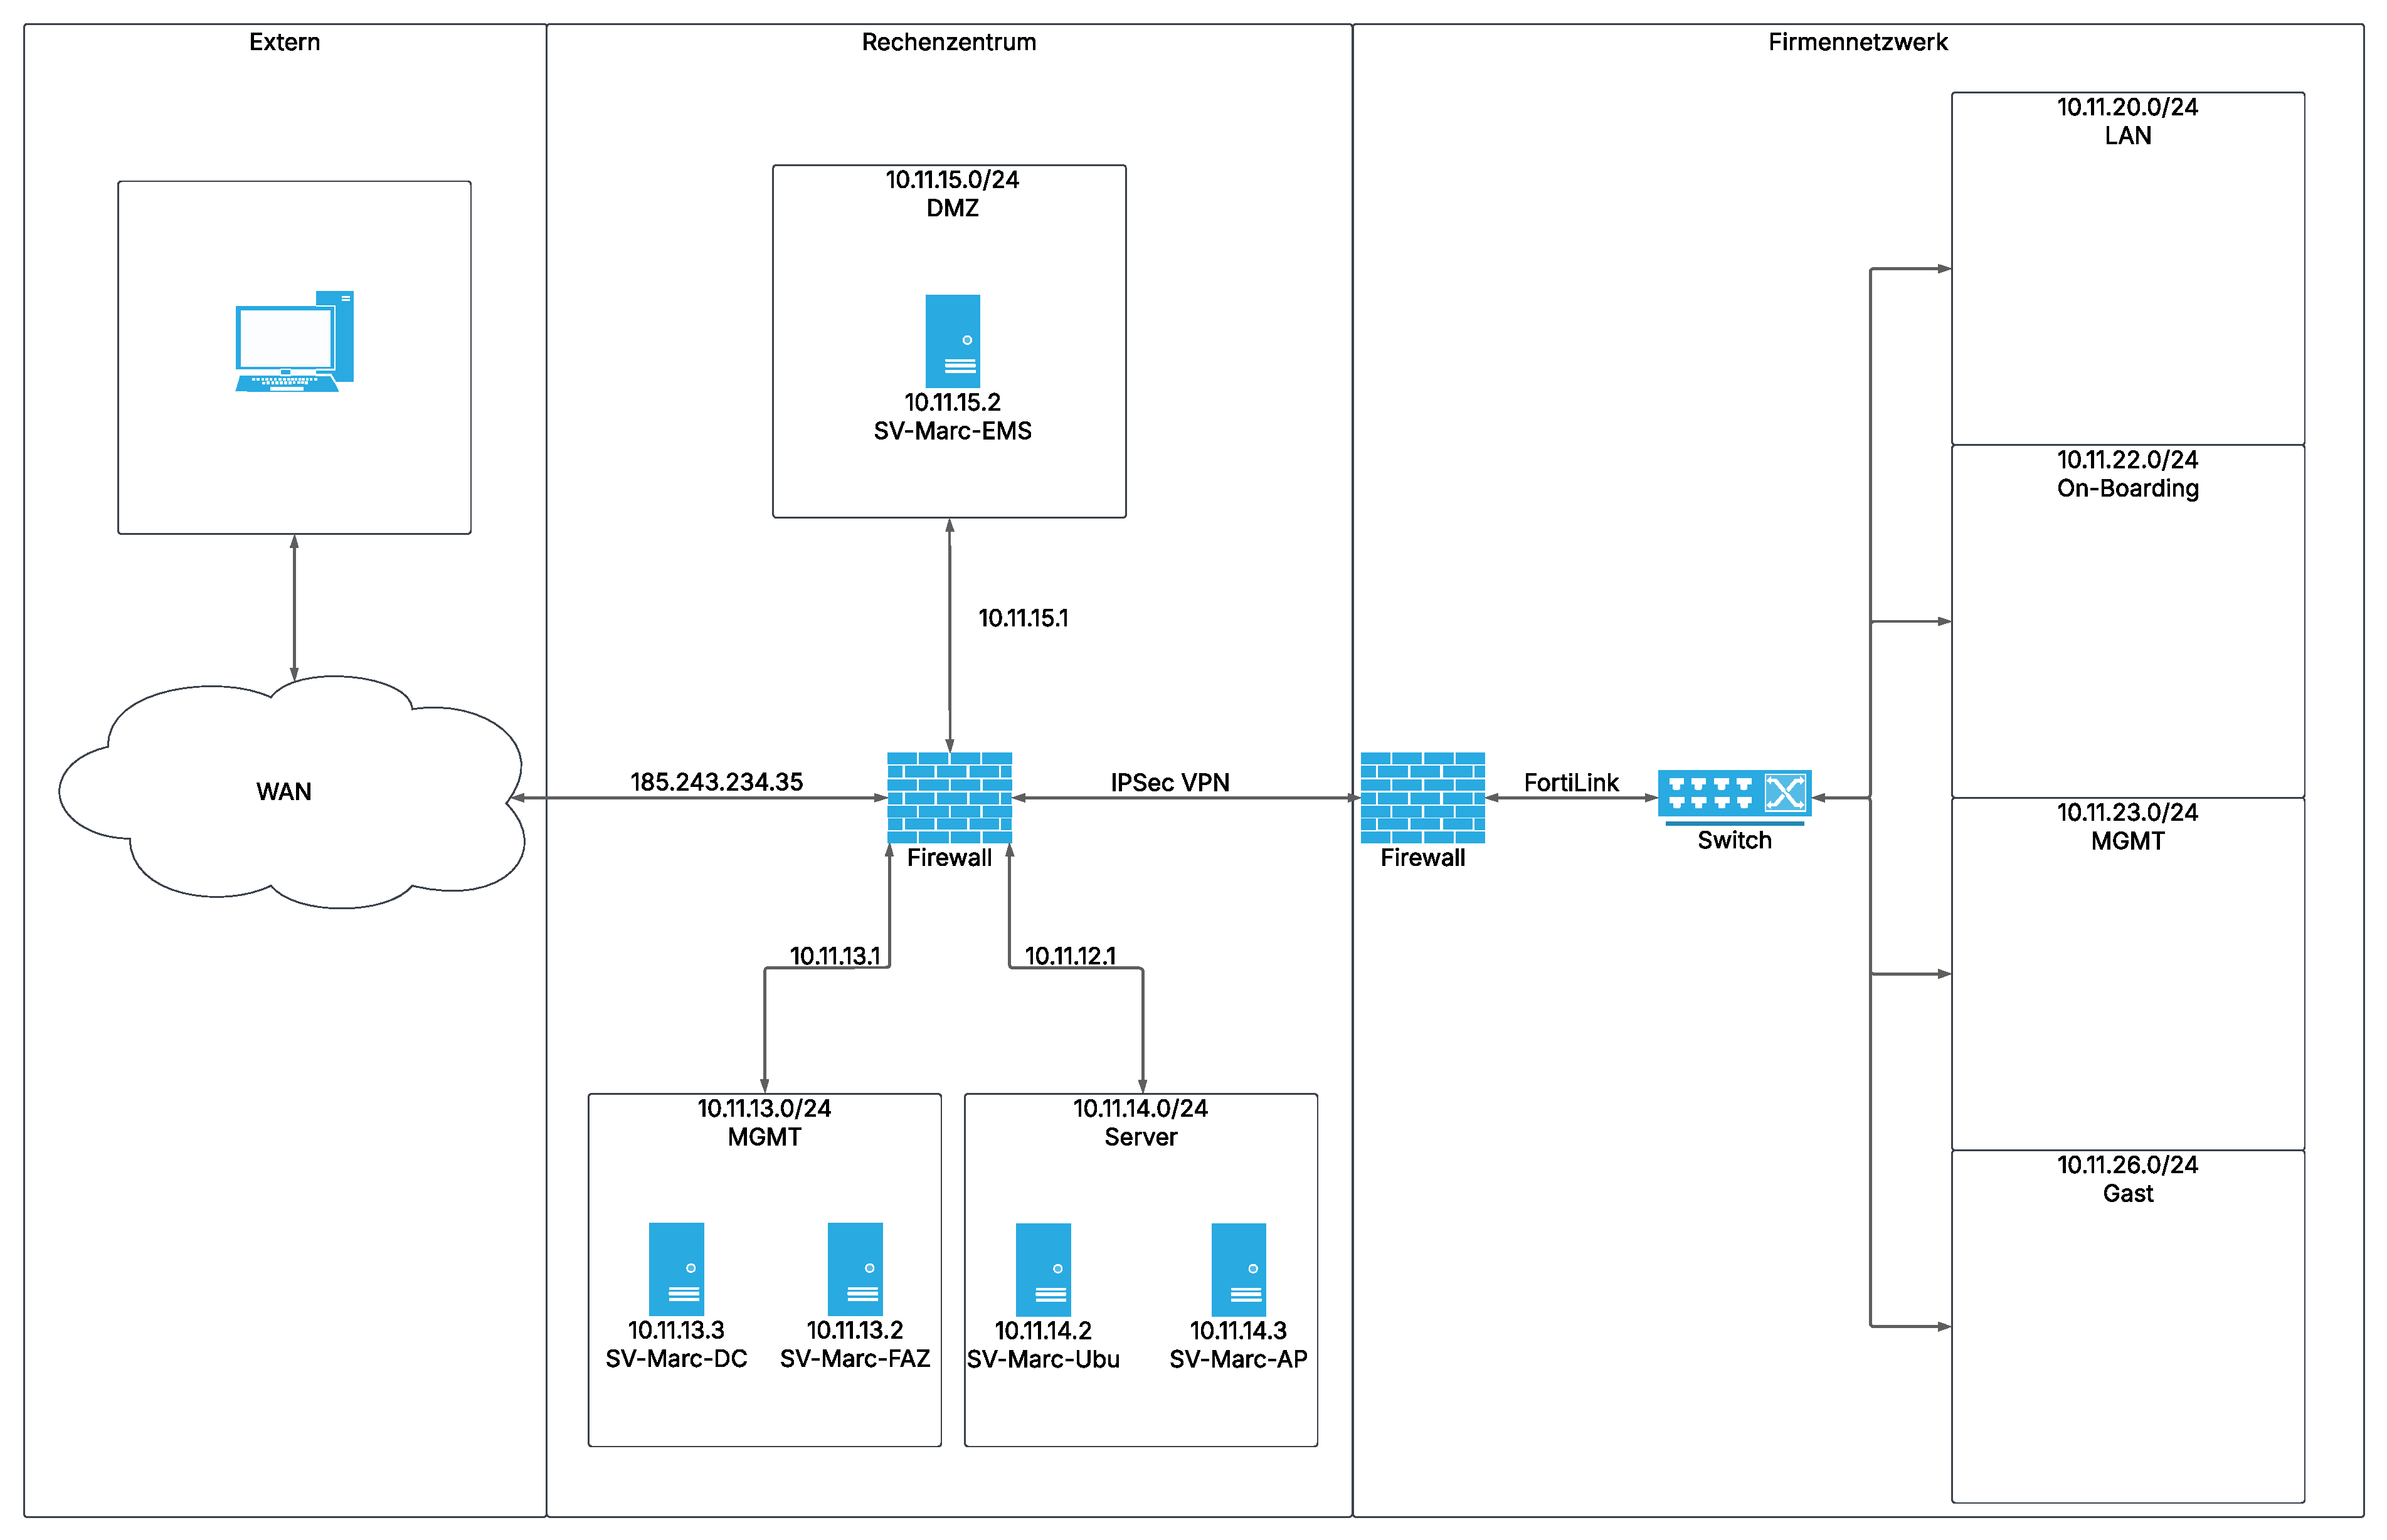
\includegraphics[width=0.9\textwidth]{Netzwerk-Topologie.pdf}
	\caption{Netzplan des Zero-Trust-Network}
	\label{fig:netzplan}
\end{figure*}

\section{Stand der Umsetzung}
Nachdem nun die ausgewählten Schlüsselkonzepte genauer genannt wurden, wird im Folgenden deren Implementierung in ein beispielhaftes Netzwerk erläutert. Bei dem beispielhaften Netzwerk handelt es sich um ein hybrides Netzwerk. Es besteht aus einem internen Firmennetzwerk, das über einen IPSec-VPN-Tunnel mit einem externen Rechenzentrum verbunden ist (siehe Abbildung 1).\\
Das interne Firmennetzwerk ist in mehrere VLANs aufgeteilt, darunter die VLANs für LAN, Onboarding, Management und Gast. Diese Segmentierung soll eine logische Trennung der Netzwerke nach Aufgabenbereichen schaffen.
Das LAN-VLAN dient dem operativen Betrieb. In diesem VLAN befinden sich Endgeräte, die mit dem Rechenzentrum kommunizieren müssen. Hier herrscht eine strenge Sicherheitspolitik. Die Zugriffe auf Ressourcen aus dem Rechenzentrum werden anhand des Endgeräts und des angemeldeten Benutzers gesteuert. Zu den Eigenschaften des Endgeräts und des angemeldeten Benutzers kommt ein Zeitplan hinzu. Dieser Zeitplan sagt aus, dass Zugriffe auf das Rechenzentrum nur innerhalb einer festgelegten Uhrzeit geschehen dürfen.
Das Onboarding-VLAN ist für die Aufnahme neuer Endgeräte in den produktiven Betrieb gedacht. Die Sicherheitspolitik hier ist noch nicht ganz so streng. Endgeräte können sich hier zunächst Informationen aus Gruppenrichtlinien und Zertifikate ziehen. Diese Informationen werden später für die Aufnahme in das LAN benötigt.
Das Management-VLAN ist als ein Kommunikationsnetzwerk gedacht. Hier kann die Firewall Ressourcen aus dem Rechenzentrum abfragen und verwalten. Ein Zugriff auf dieses Netzwerk ist ohne Weiteres nicht möglich. Eine Verbindung mit diesem Netzwerk ist nur als Emergency-Plan gedacht, wenn die Sicherheitskomponenten im Rechenzentrum versagen und es keinen Zugriff mehr aus dem LAN in Richtung Rechenzentrum gibt.
Das Gast-VLAN ist für alle Endgeräte, die nicht am operativen Betrieb der Firma teilnehmen. Angedacht ist dieses Netzwerk für beispielsweise Smartphones oder sonstige unbekannte Endgeräte. Dieses VLAN ist das standardmäßige Netzwerk, in dem zunächst alle Endgeräte kommen.
Eine Erweiterung der VLANs ist jederzeit möglich. Beispielsweise kann ein separates VLAN für IoT-Endgeräte angelegt werden, welches nur eingeschränkten oder gar keinen Internetzugriff besitzt.\\
Auch das Netzwerk im Rechenzentrum ist in mehrere VLANs aufgeteilt. Die logische Trennung der Netzwerke erfolgt in VLANs für Server, eins für Management und eins für die demilitarisierte Zone.
Das Servernetz ist für verschiedene Arten von Servern angedacht. Hier befinden sich die Ressourcen des Unternehmens. Typische Serverkomponenten können Webserver, Terminalserver, Applikationsserver und Datenbanken sein. Im beispielhaften Netzwerk ist aus Gründen der Einfachheit nur ein Webserver zu finden. Das Managementnetzwerk im Rechenzentrum ist speziell für die Verwaltung, Wartung und Überwachung der einzelnen Netzwerkkomponenten gedacht. Zusätzlich zum Domänencontroller ist der Fortinet FortiAnalyzer in diesem Netzwerk zu finden. Der FortiAnalyzer ist für die Überwachung und Analyse des Netzwerkes zuständig. Er hat Zugriff auf alle Ereignisprotokolle, die von den Fortinet FortiGates und dem FortiClient Endpoint Management Server kommen. Als letztes logisches Netzwerk ist die demilitarisierte Zone angedacht. Obwohl die Zero Trust Philosophie aussagt, dass Netzwerkbereiche implizit nicht vertrauenswürdig sind und eine Trennung von internen und externen Zonen somit überflüssig erscheint, wurde sich dennoch für die Konfiguration eines DMZ Netzwerkes entschieden. Der Grund der Trennung ist die Art und Weise des externen Zugriffes. In der DMZ befindet sich der FortiClient Endpoint Management Server. Dieser Server ist durch ein gezieltes Konfigurieren von Port-Forwarding Regeln extern erreichbar gemacht.\\
Innerhalb der VLANs ist es möglich, den Intra-VLAN Datenverkehr zu blockieren. Dies bedeutet, dass Endgeräte desselben VLAN nur über die Firewall miteinander kommunizieren können. Die Firewall hat so volle Sichtbarkeit über die Datenpakete des gesamten Netzwerkes. Die Kommunikation von Endgeräten eines VLAN muss, wie auch die Kommunikation mit Endgeräten außerhalb des eigenen VLANs, explizit erlaubt werden. Die zentralen Komponenten dieses Netzwerkes sind die FortiGate Firewalls, der FortiClient Endpoint Management Server und der FortiAnalyzer. Im Rahmen der Implementierung wurde ein besonderes Augenmerk auf diese Komponenten geworfen, um die Schlüsselkonzepte des Zero Trust Network umzusetzen.

\subsection{FortiGate Firewall}
Bei der FortiGate Firewall handelt es sich um eine Next-Generation-Firewall (NGFW). Die Next-Generation-Firewalls haben im Gegensatz zu gewöhnlichen Firewalls mehr Features. Eine gewöhnliche Firewall analysiert eingehende und ausgehende Datenpakete hinsichtlich vorher definierter Sicherheitsrichtlinien. Diese Sicherheitsprüfung führt dazu, dass Pakete, die nicht den definierten Richtlinien entsprechen, verworfen werden. Zudem wird der Kontext der Pakete berücksichtigt. Pakete müssen Teil einer legitimen Netzwerkverbindung sein. Außerdem bieten gewöhnliche Firewalls eine Schnittstelle für die Nutzung eines Virtual-Private-Network (VPN). Next-Generation-Firewalls erweitern den Umfang an Sicherheitsfeatures erheblich. Sie verfügen über Application-Awareness und ermöglichen damit die gezielte Kontrolle von Anwendungen. Durch Deep-Packet-Inspection (DPI) analysieren sie auch den Payload von Datenpaketen. Sicherheitsrelevante Inhalte oder Muster können so erkannt werden. Zusätzlich integrieren NGFWs Funktionen zur Intrusion-Prevention (IPS), mit denen bekannte Angriffe in Echtzeit erkannt und verhindert werden können. Dank der Threat-Intelligence kann ein Abgleich mit Bedrohungsdatenbanken erfolgen, sodass verdächtiges Verhalten frühzeitig identifiziert werden kann. Um diese Firewalls auf dem neuesten Stand zu halten, bieten sie eine Schnittstelle für spätere Upgrades an. Damit lassen sich künftige Informations-Feeds und neue Techniken zur Abwehr von Bedrohungen flexibel integrieren. Dies ermöglicht eine dynamische Sicherheitsplattform, die auch angesichts sich ständig weiterentwickelnder Bedrohungen eine robuste Verteidigung bietet \cite{cloudflare.com.20250625}.\\
Im Rahmen der praktischen Implementierung eines Zero Trust Network wurden die Firewalls als zentrale Komponente zur Umsetzung der Schlüsselkomponenten konfiguriert. Dabei kamen zahlreiche NGFW-Funktionen zum Einsatz. Ein wesentlicher Bestandteil war dabei das Konfigurieren der SSL-Deep-Inspektion. Der Großteil des Datenverkehrs im Internet erfolgt heute über HTTPS. Dabei wird eine verschlüsselte Verbindung zwischen den beiden Kommunikationspartnern hergestellt. Dank der SSL-Deep-Inspektion kann die Firewall auch diesen auf böswilligen Inhalt prüfen. Zusätzlich wurden mehrere Security-Profile eingebunden, darunter Antivirus, IPS und Application-Control. Des Weiteren wurde die Konfiguration der Policies so vorgenommen, dass sie sich nicht nur auf IP-Adressen und Services beschränkt. Policies berücksichtigen bei der Auswertung zusätzlich die genannten Security-Profile. Zudem wurden bei den Policies sogenannte Tags verwendet. Diese Tags werden, nach Prüfung bestimmter Voraussetzungen, vom EMS-Server an ein Endgerät ausgestellt. Diese Tags dienen als Erweiterung von Merkmalen, die geprüft werden können.
Ein weiterer wesentlicher Bestandteil war das Konfigurieren des Zero Trust Network Access Proxys. Dieser Proxy ersetzt die klassische Verwendung eines VPN-Zugangs. Externe Anfragen werden dabei über einen Proxy an interne Ressourcen weitergeleitet. Die Weiterleitung basiert dabei auf einer identitäts- und richtlinienbasierten Sicherheitsprüfung. Die FortiGate ermöglicht zudem das Umsetzen einer NAC-Policy. Dabei kann anhand von Endgeräteinformationen entschieden werden, ob das Endgerät in ein bestimmtes Netzwerk kommt oder nicht. Diese Entscheidung basiert auch auf den Tags. Die FortiGate erfüllt die technischen Maßnahmen zur Umsetzung des Zugriffsmanagements und der Netzwerkzugriffskontrolle.

\subsection{FortiClient Endpoint Management Server}
Eine weitere zentrale Komponente ist der FortiClient Endpoint Management Server. Der EMS-Server hat die Aufgabe, Endgeräte zu erfassen und diese kontinuierlich zu überwachen. Dazu wird auf dem Endgerät ein FortiClient installiert. In regelmäßigen Abständen findet eine sogenannte Telemetrieverbindung statt. Dabei sendet der FortiClient endgeräte- und nutzerspezifische Informationen an den EMS-Server. Basierend auf diesen Daten kann der EMS-Server sogenannte Tags vergeben. Diese Tags dienen als Zusatzmerkmal und können bei der FortiGate Firewall für Zugriffsentscheidungen berücksichtigt werden. Der EMS-Server schafft zudem die Grundvoraussetzung für den ZTNA-Zugriff. Die Voraussetzung zur Nutzung des ZTNA-Proxys ist die vorher hergestellte Verbindung mit dem EMS-Server. Das bedeutet, dass der EMS-Server auch von extern erreicht werden muss. Dies ist der Grund für die Konfiguration einer DMZ Zone. Der Endpoint Management Server ist im Datenaustausch mit dem Domänencontroller. So kann sichergestellt werden, dass der EMS-Server alle Domänenbenutzer kennt. Neben dem Identifizieren und Kategorisieren der Endgeräte kann der EMS-Server auch als Zentrale zum Ausrollen von Richtlinien und Patches verwendet werden. Dabei können im EMS-Server Policies erstellt werden, die gruppenspezifisch sind. Dies ermöglicht beispielsweise eine Restriktion der Nutzung des Internets, auch wenn das Endgerät nicht im internen Firmennetzwerk ist.\\
Im Rahmen der Implementierung wurde eine Verbindung zwischen dem EMS-Server und der FortiGate hergestellt. Diese Verbindung sorgt dafür, dass die FortiGate stets über den aktuellen Endgerätezustand informiert ist. Die FortiGate kann so immer auf Grundlage aktueller Kriterien Entscheidungen treffen. Zudem ist der EMS-Server mit dem Domänencontroller verbunden, um Informationen über Benutzerinformationen wie Gruppenzugehörigkeit abfragen zu können. Auf Grundlage dieser Informationen wurden rollenbasierte Policies erstellt. Diese Policies werden dann direkt auf den Endgeräten umgesetzt. Dazu zählen Webfilter und die Konfiguration des ZTNA-Proxy. So kann ein Webfilter auch angewendet werden, wenn das Endgerät nicht im internen Firmennetzwerk ist. Die Policies für den Proxy sorgen für eine automatische Weiterleitung. 
Der Benutzer gibt dabei die interne IP-Adresse ein. Die Policy sorgt dafür, dass diese interne IP-Adresse auf den externen Proxy umgeleitet wird. Nach erfolgreicher Sicherheitsprüfung hat der Benutzer Zugriff auf die interne Ressource. Nutzer merken die Weiterleitung nicht. Damit eine Verbindung mit dem ZTNA-Proxy möglich ist, muss das Endgerät mittels des FortiClient mit dem EMS-Server verbunden sein. Diese Verbindung ist der Grund, warum der EMS-Server von extern erreichbar gemacht wurde. Der FortiClient Endpoint Management Server erfüllt die technischen Maßnahmen zur Umsetzung der Gerätesicherheit und des Identitätsmanagements und bietet die Grundlage für eine Erweiterung des Zugriffsmanagements.

\subsection{Fortinet Analyzer}
Der Fortinet Analyzer ergänzt das Zero Trust Network um ein zentrales Monitoring- und Auswertungstool. Der FortiAnalyzer dient primär der Sammlung aller Ereignisse in Form von Logs innerhalb des Netzwerkes. Mittels dieser Ereignisse kann der FortiAnalyzer sicherheitsrelevante Ereignisse filtern und notwendige Handlungen umsetzen.\\
Im Rahmen der praktischen Umsetzung wurde der FortiAnalyzer so konfiguriert, dass er Logs beider FortiGate Firewalls und des EMS-Servers bekommt. Das Netzwerk ist so konfiguriert, dass jeder Zugriff über die Firewall laufen muss. Entsprechend hat der FortiAnalyzer volle Sichtbarkeit in das gesamte Netzwerk. Die Auswertung der Logs erfolgt über individuell konfigurierbare Reports, sodass sicherheitsrelevante Vorfälle frühzeitig erkannt werden. Der FortiAnalyzer hat zudem die Möglichkeit, ein Event auf Grundlage von Triggern auszulösen. Trigger können dabei Sicherheitsverstöße sein. So wurde konfiguriert, dass wenn sich ein Endgerät böswillig verhält, die FortiGate informiert wird und das Endgerät per Network Access Control in einen Quarantänezustand versetzt wird. So können Endgeräte dynamisch in Isolation versetzt werden.


\section{Ausblick}
Die Implementierung bietet eine solide Grundlage, auf die weiter aufgebaut werden kann. Ein nächster logischer Schritt wäre die Einbindung an Azure Active Directory. Azure AD ermöglicht Benutzeridentifikation auf Cloudbasis. Zudem ist die Einbindung von Single-Sign-On mittels Azure AD möglich. Dies würde die Benutzerfreundlichkeit, aber auch die Sicherheit erhöhen. Ein weiterer Schritt wäre die Implementierung eines vollständigen NAC-Systems. Zwar sind die Grundlagen eines NAC-Systems enthalten und die dynamische Zuweisung von VLANs vorhanden, ein vollständiges NAC-System würde jedoch eine präzisere Steuerung für nicht konforme Endgeräte wie beispielsweise IoT-Endgeräte ermöglichen. Auch im Bereich des Monitorings ist eine Erweiterung der Reports möglich. Dies würde eine Verbesserung der Sicherheitsmaßnahmen bedeuten, da der FortiAnalyzer detaillierte Benutzerzugriffsanalysen erstellen könnte. Insgesamt ist die aktuelle Umsetzung eine sehr praxisnahe, die sich jederzeit modular erweitern lässt.

\section{Fazit}
Die vorliegende Umsetzung zeigt die Konzeption eines Zero Trust Network in einer hybriden IT-Infrastruktur. Ausgangspunkt war die zunehmende mangelnde Eignung des klassischen, parameterbasierten Sicherheitsmodells in modernen und dynamisch sich verändernden Unternehmensnetzwerken. Mit den Zero Trust Prinzipien konnte ein Sicherheitskonzept umgesetzt werden, das sich flexibel an Bedingungen anpasst und auf kontinuierlicher Prüfung der Identität und des Kontexts basiert.\\
Im praktischen Teil der Arbeit erfolgte die Implementierung eines beispielhaften hybriden Unternehmensnetzwerkes. Herzstück der Implementierung waren die FortiGate Firewalls im Rechenzentrum und im internen Firmennetzwerk. Mittels dieser Firewalls war es unter anderem möglich, die einzelnen Netzwerke in logische, voneinander getrennte VLANs aufzuteilen. Nach der Trennung wurden in den verschiedenen Zonen weitere Komponenten wie der Domänencontroller, der FortiClient Endpoint Management Server und der Fortinet FortiAnalyzer konfiguriert. Die Integration dieser Systeme bildet eine Grundlage, um die wesentlichen Schlüsselkomponenten Zugriffskontrolle, Gerätesicherheit, Netzwerksegmentierung sowie Monitoring und Überwachung zu erfüllen.\\
Die Implementierung verdeutlicht, dass Zero Trust nicht durch die Integration eines einzelnen Produktes realisiert werden kann. Vielmehr ist Zero Trust eine gezielte Kombination aus verschiedenen Systemen, Richtlinien und kontinuierlicher Neubewertung. Dabei ist Zero Trust ein Ansatz, der bei jeder Integration neuer Systeme beachtet werden muss. Die aktuelle Architektur bietet bereits ein hohes Maß an Sicherheit und ist zugleich so strukturiert, dass weitere Komponenten modular erweitert werden können. Beispielsweise durch die Anbindung von Azure Active Directory.\\
Die Arbeit liefert nicht nur eine theoretische Auseinandersetzung mit der Zero Trust Thematik, sondern auch eine praktische Realisierbarkeit und Weiterentwicklung in einer hybriden Netzwerkinfrastruktur.


\bibliographystyle{IEEEtran}
\bibliography{main}

\end{document}
